% !TEX root = demo.tex
\section{System Architecture}

In this section, we provide a brief overview of \sys and how it fits into
the AMPLab big data stack.
The subsequent sections describe the logical operators, the cleaning language,
and the implementation details, including the physical operator implementations.

Figure~\ref{fig:arch} depicts the highlight system architecture and the API. 
The left subfigure shows \sanjay{describe query execution flow}.

  \begin{figure*}[ht]
  \centering
  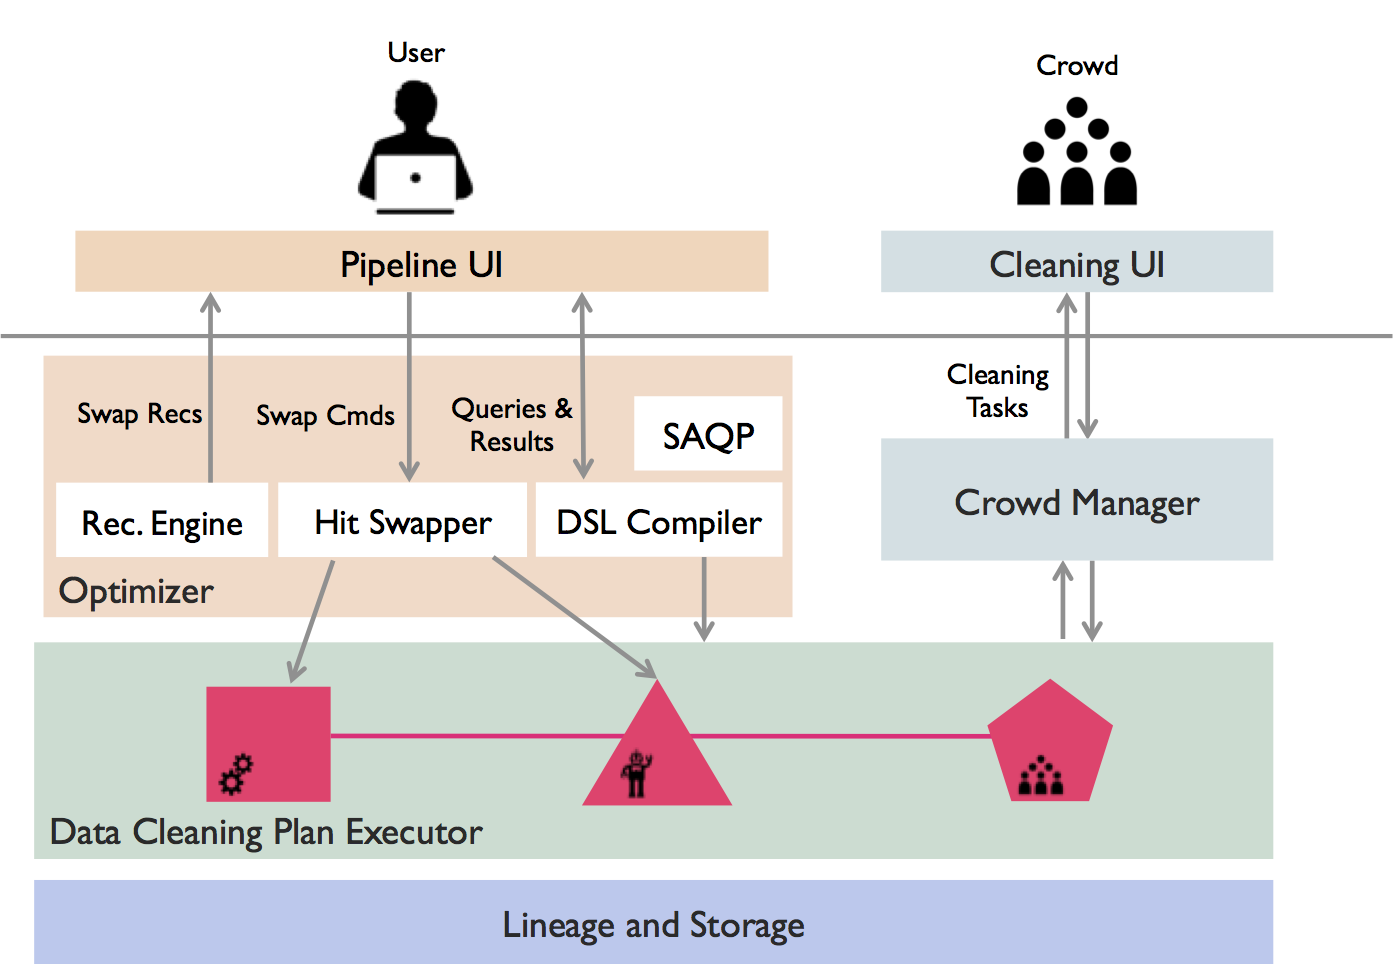
\includegraphics[width = \textwidth]{figs/architecture.png}
  \caption{\sys system architecture.}
  \label{fig:arch}
  \end{figure*}


\subsection{Language Overview}
We provide a language for specifying the composition of data cleaning operators.
The logical operators define the input and output behavior of the operation and 
the physical operators specify the implementation.
The general syntax of this language is:
\begin{lstlisting}
<logical operator> on <relations>
	with <physical operators> , <params>
\end{lstlisting}
\ewu{Why or when is WITH clause necessary? }
These expressions are composable:
\begin{lstlisting}
R1 := <logical operator> on <relations> 
	with <physical operators> , <params>
R2 := <logical operator> on R1 
	with <physical operators> , <params>
\end{lstlisting}
\projx provides an integration layer of these expressions with Scala/Apache Spark allowing for the manipulation of SchemaRDDs (Spark RDDs with additional schema information):
\begin{lstlisting}
val rddA = spark.textFile(file).toSchemaRDD
val cleanData = clean(rddA,<expression>)
\end{lstlisting}


\subsection{Data and Execution Model}

\team{fill in}

Each operator is treated like a view?

Execution is a tree/graph/line/dag.


